\chapter{Deterministic Mean Field Particle Systems}
\begin{definition}[Deterministic Mean Field Particle System]
  For $N \in  \mathbb{N}$ a deterministic mean field particle system is given by N particles : 
  \begin{align*}
   x_1(t),\ldots ,x_n(t) \in  \mathcal{C}^{1}([0,T];\mathbb{R}^{d } )  \qquad x_i(0) = c_i
  .\end{align*}
  With initial points : 
  \begin{align*}
    x_i(0) = x_{i,0} \in \mathbb{R}^{d} 
  .\end{align*}
  And the relation : 
  \begin{align*}
    \frac{d}{dt} x_{i} = \frac{1}{N} \sum_{j=1}^{N}  K(x_i,x_{j})
  .\end{align*}
  The system is then given by : 
  \begin{align*}
    X_N = \begin{pmatrix} x_1(t) \\ x_2(t) \\ \vdots \\ x_N(t)  \end{pmatrix} \in \mathbb{R}^{dN} 
  .\end{align*}
\end{definition}
The goal is to solve the above $d*N$ dimensional system under assumptions on K.
\section{ODE Theory}
\begin{definition}[Initial Value Problem (standard)]
 For $\forall  T > 0 $  the standard ode system is given by : 
 \begin{align*}
  x' &= f(t,x) \\
  x \vert_{t=0} &=  x_0 \in \mathbb{R}^{n} 
 .\end{align*}
 with $t \in  [0,T] ,\ x(t) \in  \mathbb{R}^{n} $
\end{definition}
\begin{assumption}[A]\label{eq:Assumption_A}
  Condition for global existence : f is continuous in $(t,x) \in  [0,T] \times \mathbb{R}^{n} $ \\ 
  Condition for uniqueness : f is Lipschitz continuous in $x$  
\end{assumption}
\begin{theorem}[]
  Whenever assumption \ref{eq:Assumption_A} holds the standard IVP has a unique solution $x \in  \mathcal{C}^{1}([0,T] ; \mathbb{R}^{n} ) $
\end{theorem}
\begin{proof}[Proof]
  Rewriting the IVP using integration : 
  \begin{align*}
    x(t) - x(0) = \int_0^{t }f(s,x(s)) ds   \quad \forall  t \in  [0,T]
  .\end{align*}
  We construct the following sequence by : 
  \begin{align*}
    x_1(t) &= x_0 + \int_0^{t }f(s,x_0) ds \\
    x_{2}(t) &= x_0 + \int_0^{t} f(s,x(s)) ds 
             &\vdots \\
    x_m(t) &= x_0 + \int_0^{t} f(s,x_{m-1}(s)) ds 
  .\end{align*}
  Step 1 of the proof consists of proving the above sequence is converging , step 2 is then showing the limit is a solution to the IVP\\[1ex]
  Under Assumption \ref{eq:Assumption_A} we know that $f$ is continuous such that $(x_n)_{n \in  N} \subset \mathcal{C}^{1}([0,T];\mathbb{R}^{n} ) $, 
  As $\mathcal{C}^{1} $ is complete any sequence that is cauchy must also converge against a limit in the space. \\[1ex]
  \begin{align*}
    \abs{x_2 - x_1} &= \abs{\int_{0}^{t} f(s,x_{1}(s)) ds  -  \int_{0}^{t} f(s,x_{0}(s)) ds  } = \abs{\int_{0}^{t} f(s,x_{m-1}(s))  - f(s,x_{n-1}(s)) ds } \\
                    &\le \int_0^{t} \abs{f(s,x_{1}(s)) - f(s,x_{0}(s))} ds    \\ 
                    &\myS{Lip.}{\le }  L \int_0^{t} \abs{x_{1}(s) - x_{0}(s) } ds  \\
                    &= L \int_0^{t } \abs{\int_0^{s_0} f(s,x_0) ds} ds_0  \\
                    &\le L * \int_0^{t} \int_0^{s_0} \abs{f(s,x_0)} ds ds_0  \\
                    &\le L \underbrace{M}_{=\max_{s \in  [0,T]}\abs{f(s,x_0)}} \frac{t^2}{2}  
  .\end{align*}
  By repeatedly using  the Lipschitz continuity of f the following induction assumption is motivated : 
  \begin{align*}
    \abs{x_m(t) - x_{m-1}(t)} \le M L^{m-1} \frac{t^m}{m!}  \tag{IA}
  .\end{align*}
  (IS) :  $m \to  m+1$
  \begin{align*}
    \abs{x_{m+1}(t) - x_{m}(t)} &\myS{Lip.}{\le }  L \int_0^{t} \abs{x_m(s)-x_{m-1}(s)} ds \\
                                &\myS{IA.}{\le } L \int_0^{t} \frac{M L^{m-1} s^{m}  }{m!} ds = ML^{m}  \frac{t^{m+1} }{(m+1)!}
  .\end{align*}
  For any $n,m \in  \mathbb{N}$ and assuming without loss of generality that  $n>m$ such that $n = m+p$ for $p \in  N$ : 
  \begin{align*}
    \abs{x_{n}(t) - x_{m}(t)} &= \abs{x_{m+p}(t) - x_{m}(t)} \le  \sum_{k=m+1}^{m+p}  \abs{x_k(t)-x_{k-1}(t)} \myS{Ind.}{\le } M \sum_{k=m+1}^{m+p}  \frac{L^{k-1 }T^{k}  }{k!}\\
                              &= \frac{M}{L} \sum_{k=m+1}^{m+p} \frac{(LT)^{k} }{k!}  = \frac{M}{L} \frac{(LT)^{m+1} }{(m+1)!}\sum_{k=0}^{p-1} \frac{(LT)^{k} }{k!}  \\
                              &\le \frac{M}{L} \frac{(LT)^{m+1} }{(m+1)!} e^{LT}  \xrightarrow{m\to \infty} 0 \text{  uniformly in } t \in  [0,T]
  .\end{align*}
  This shows that $(x_m)_{m \in  \mathbb{N}}$  is Cauchy and has a limit $x \in  \mathcal{C}([0,T];\mathbb{R}^{n} )$ with : 
  \begin{align*}
    \max_{t \in  [0,T]} \abs{x_m(t) - x(t)} \to  0
  .\end{align*}
  It remains to show that $x(t)$ is a solution to the IVP i.e : 
  \begin{align*}
    x(t) =  \lim_{m\to \infty} x_0 + \int_0^{t} f(s,x_{m-1}(s)) ds  \leftrightarrow x_0 + \int_0^{t} f(s,x(s)) ds 
  .\end{align*}
 Which can be shown by : 
 \begin{align*}
   \abs{\lim_{m \to \infty} \int_0^{t} f(s,x_{m-1}(s))  - f(s,x(s)) ds } &\le  \lim_{m \to  \infty} \int_0^{t} \abs{f(s,x_{m-1}(s))-f(s,x(s))} ds \\
                                                                         &\le  \lim_{m \to \infty} L \int_0^{t} \abs{x_{m-1}(s)-x(s)} ds \\
                                                                         &\le  \lim_{m \to \infty} L t*\max_{s \in [0,t]} \abs{x_{m-1}(s) x(s)}\\
                                                                         &\le   \lim_{m \to \infty} L t*\max_{s \in [0,T]} \abs{x_{m-1}(s) x(s)}\\
                                                                         = 0 
 .\end{align*}
 It remains to show that the solution is unique, for that assume $x,\hat{x}  \in  \mathcal{C}([0,T];\mathbb{R}^{n} )$ are both solutions to the IVP.
 Meaning that : 
 \begin{align*}
   x(t) &= x_0 + \int_0^{t} f(s,x(s)) ds \\
   \hat{x}(t) &= x_0 + \int_0^{t} f(s,\hat{x}(s) ) ds  
 .\end{align*}
 Then : 
 \begin{align*}
   \abs{x - \hat{x} } &\le  \int_0^{t} \abs{f(s,x(s))-f(s,\hat{x}(s) )} ds \le  L * \int_0^{t} \abs{x(s) - \hat{x}(s) } ds  \\
                      &=  L \int_0^{t} \underbrace{e^{-\alpha s} \abs{x(s)-\hat{x}(s) }}_{=\rho(s)} e^{\alpha s} ds \\
                      &\le  L \max_{t \in  [0,T]} \rho(t) * \frac{1}{\alpha } (e^{\alpha t} - 1) \\
                      &\le  L \max_{t \in  [0,T]} \rho(t) * \frac{1}{\alpha }* e^{\alpha t} 
 .\end{align*}
By rearranging with the initial term : 
\begin{align*}
  \rho(t) = e^{-\alpha t} \abs{x(t)-\hat{x}(t) } &\le \frac{L}{\alpha } \max_{t \in [0,T]} \rho(t) \\
  \max_{t \in  [0,T]} \rho(t) \le  \frac{L}{\alpha } \max{t \in  [0,T]} \rho(t)
.\end{align*}
by choosing $\alpha = 2L$ : 
\begin{align*}
  \max_{t \in  [0,T]} e^{-2Lt} \abs{x(t)-\hat{x}(t) } = 0 
.\end{align*}
And the solutions must be equal for $\forall  t \in  [0,T]$.
\end{proof}
\hspace{0mm}\\
The reason this proof deviates from the standard Picard-Lindelöf theorem, is that for our systems we require Global existence, doing so by requiring $f$ to be globally Lipschitz continuous.
\begin{theorem}
  The solution $x(t,t_0,x_0) \in  \mathcal{C}$ is continuously dependent on $(t_0,x_0)$
\end{theorem}
\begin{theorem}[Gronwalls inequality]
  For $\alpha ,\beta ,\phi  \in  \mathcal{C}([a,b];\mathbb{R})$  $\beta \ge 0$ and 
  \begin{align*}
    0\le \phi(t) \le  \alpha(t) + \int_a^{t} \beta(s) \phi(s) ds , \ \forall t \in [a,b]
  .\end{align*}
  then : 
  \begin{align*}
    \phi(t) \le \alpha(t) + \int_{a}^{t} \beta(s) \exp\left(\int_s^{t} \beta(\tau ) d\tau   \right)  \alpha(s) ds
  .\end{align*}
\end{theorem}
\begin{proof}[Proof]
  Denote $\psi(t) = \int_a^{t} \beta(s) \phi(s) ds $ then 
  \begin{align*}
    \psi'(t) &= \beta(t)\phi(t) \le \beta(t)\alpha(t) + \beta(t)\psi(t) \\
             &= \beta(t) * (\alpha(t) + \psi(t))\\
  .\end{align*}
  Recall $\dot{x} + a(t)x + b(t) = 0$
  \begin{align*}
    (\dot{\psi}(t) - \beta(t)\psi(t) )e^{- \int_a^{t}\beta(s) ds } &\le  \beta(t)\alpha(t)*e^{-\int_a^{t} \beta(s) ds } \\
    (e^{- \int_a^{t}\beta(s) ds } \psi(t))' &\le \beta(t) \alpha(t)*e^{-\int_a^{t} \beta(s) ds } 
  .\end{align*}
  Integrating gives : 
  \begin{align*}
    (e^{- \int_a^{t}\beta(s) ds } \psi(t)) \myS{$\psi(a) =0$}{\le } \int_a^{t} \beta(s) \alpha(s) e^{-\int_a^{s}\beta(r) dr } ds  
  .\end{align*}
\end{proof}
\begin{definition}[Regularity]
  A function $K : \mathbb{R}^{2d} \to \mathbb{R}^{d}  $ is called regular if :
  \begin{enumerate}
    \item $K \in  \mathcal{C}^{1}(\mathbb{R}^{2d};\mathbb{R}^{d}  ) $ (gives local lipschitz ) 
    \item And $\exists  L >0 $ s.t. : 
      \begin{align*}
        \sup_{y} \abs{\triangledown_x K(x,y) } + \sup_{x} \abs{\triangledown_y K(x,y)}  \le L
      .\end{align*}
  \end{enumerate} 
\end{definition}
We further assume $K$ has the following properties :
\begin{align*}
  K(x,y) &= -K(y,x) \tag{antisymmetric}\\
    K(x,x) &= 0 
.\end{align*}
 \begin{theorem}
 When the assumption of regularity on $K$  holds, the MPS has a solution for all $T>0$
\begin{align*}
  \begin{cases}
    \frac{d}{dt} x_i &= \frac{1}{N} \sum_{j=1}^{N} K(x_i,x_j) ,  1\le i \le N \\ 
    x_i(0)  &= x_{i,0} \in \mathbb{R}^{d} 
  \end{cases}
 .\end{align*}
 has a unique solution by Picard-Iteration : 
 \begin{align*}
   X_N(t) = \begin{pmatrix} x_1(t),x_2(t),\ldots ,x_N(t) \end{pmatrix}  \in \mathcal{C}^{1}([0,T];\mathbb{R}^{dN} ) 
 .\end{align*}
 \end{theorem}

 \begin{definition}[Empirical Measure of a System]\label{empirical_measure}
  Consider the point measure for every $x_i : \delta_{x_{i}(t)}$ , then the measure of the System of order N is given by
 \begin{align*}
   \mu_N(t) = \frac{1}{N} \sum_{i=1}^{N} \delta_{x_{i}(t)}
 .\end{align*}
\end{definition}
As shown in the introduction $\mu_N$ is a (weak-) solution to the  following PDE 
\begin{align*}
  &\partial_t \mu_N + \triangledown * (\mu_N * \int K(\cdot,y)d \mu_N(y)) = 0
  .\end{align*}
\begin{idea}
  Now for $N\to \infty$ if we have $\mu_N \xrightarrow{\text{in some sense}} \mu $   then $\mu $ is a (weak) solution to 
  \begin{align*}
    \partial_t \mu + \triangledown * (\mu * \int K(\cdot,y)d \mu(y)) = 0
  .\end{align*}
  with 
  \begin{align*}
    \mu_0 \leftarrow \mu_N(0)
  .\end{align*}
\end{idea}
\section{Weak Solutions and Distributions}
Distributions are a more general class of functions and can be seen as the dual space of the space of test functions 
\begin{definition}[Multi-Index]
A multi-index $\gamma \in \N_0^n$ of length $\abs{\gamma } = \sum_{i} \gamma_i$
for example $\gamma  = (0,2,1) \in \N^3_0$  can be used to denote partial derivatives of higher order as such : 
\begin{align*}
  \partial^{\gamma } = \prod_i (\frac{\partial}{\partial x_i})^{\gamma_i}
.\end{align*}
\end{definition}
\begin{myblock}
Only sensible cause partial derivatives commute as otherwise the index would be ambiguous.
\end{myblock}  
\hspace{0mm}\\
\begin{definition}[Test Functions]
 For $\Omega \subset  \mathbb{R}^{d} $  the space of test functions \\ $\mathcal{D}(\Omega) \supset \mathcal{C}_0^{\infty}(\Omega) $.
 We say a sequence of test functions $(\phi_m)_{m \in  \mathbb{N}} \subset \mathcal{C}_0^{\infty}(\Omega )$ converges against some limit $\phi \in  \mathcal{C}_0^{\infty}(\Omega ) $ iff.
 \begin{enumerate}
  \item $\exists $ a compact set $K \subset  \Omega $ s.t. $\supp \phi_m \subset  K$ for all $m \in  \mathbb{N}$ 
  \item $\forall $ multi-indexes $\alpha \in  \mathbb{N}_0^{n}  $ :
    \begin{align*}
      \sup_{K} \abs{\partial^{\alpha} \phi_m - \partial ^{\alpha } \phi   } \xrightarrow{m\to \infty} 0
    .\end{align*}
 \end{enumerate}
\end{definition}
\begin{remark}
  $\mathcal{D}(\Omega )$ is a linear space  
\end{remark}
\begin{definition}[Distribution]
  The space of distributions  $\mathcal{D}(\Omega)'$  is the dual space of $\mathcal{D}(\Omega )$ i.e. 
  $\mathcal{D}(\Omega )'$ contains all the continuous linear functionals $T$ 
  \begin{align*}
    T : \mathcal{D}(\Omega ) \to  \mathbb{K}
  .\end{align*}
\end{definition}
\begin{remark}
  Continuity  refers to the notion that for a sequence \\  $(\phi_m)_{m \in  \mathbb{N}} \subset  \mathcal{D}(\Omega )$  with limit $\phi $ then : 
  \begin{align*}
    \phi_m \to \phi  \ \implies \ T(\phi_m) \to  T(\phi )
  .\end{align*}
  linearity : 
  \begin{align*}
    T(\alpha \phi_1 + \beta \phi_2) = \alpha T(\phi_1) + \beta T(\phi_2)
  .\end{align*}
  We sometimes write $\braket{T,\phi}$ instead of $T(\phi )$
\end{remark}
\begin{definition}[Convergence]
  For a sequence of distributions $(T_m)_{m \in  \mathbb{N}} \subset  \mathcal{D}(\Omega )'$  we say it converges against a limit $T \in \mathcal{D}(\Omega)$  iff 
  \begin{align*}
    \braket{T_m,\phi } \to  \braket{T,\phi } , \quad \forall \phi  \in  \mathcal{D}(\Omega )
  .\end{align*}
\end{definition}
\begin{example}
  Every locally integrable function $ f \in  L_{\text{loc}}^{1}(\Omega ) \coloneqq  \{f \ | \ \forall K \subset  \Omega , \int_K f(x) dx < \infty \}  $  defines a Distribution by    : 
  \begin{align*}
    T_f(\phi )  = \braket{T_f,\phi } = \int_\Omega f(x) \phi(x) dx . \quad \forall \phi \in \mathcal{D}(\Omega)
  .\end{align*}
  i.e. $L_{\text{loc}}^{1}(\Omega ) \subset  \mathcal{D}'(\Omega ) $
\end{example}
\begin{example}
  Probability densities are distributions in the same sense as for $L_{\text{loc}}^{1} $ functions
\end{example}
\begin{example}
  (Probability - ) Measures $ \mu  \in  \mathcal{M}(\Omega )$ define  a distributions , by : 
  \begin{align*}
    \braket{T_\mu ,\phi } = \int_{\mathbb{R}^{d} } \phi(x) d\mu(x) < \infty \quad \forall \phi \in \mathcal{D}(\Omega)
  .\end{align*}
  A prominent example is the $\delta $ distribution defined by : 
  \begin{align*}
    \braket{\delta ,\phi } = \int_{\mathbb{R}^{d} } \phi(x) d \delta   = \phi(0)
  .\end{align*}
  \begin{myblock}
   Remember for a measurable set $E$ 
   \begin{align*}
    \delta_x(E) = \begin{cases}
      1, &\text{ if }x \in  E \\
      0  &\text{ if }x \not\in E
    \end{cases}
   .\end{align*}
  \end{myblock}
\end{example}
\hspace{0mm}\\
Coming back to our empirical measure from \ref{empirical_measure}, we can see the corresponding distribution is defined by : 
\begin{align*}
  \braket{\mu_n,\phi } = \frac{1}{N} \sum_{i=1}^{N} \phi(x_i)
.\end{align*}
Some examples in approximation of $\delta $ distribution 
\begin{example}[Heat Kernel]
  The heat kernel $f_t(x) = \frac{1}{2 \sqrt{\pi  t} } e^{- \frac{x^2}{4t}} $
  approximates the $\delta $ distribution
\begin{figure}[h]
  \begin{center}
    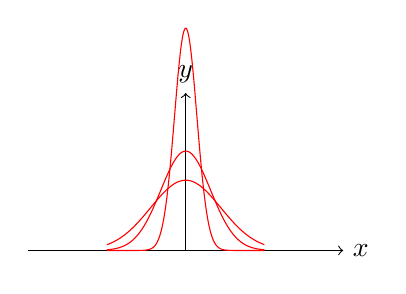
\begin{tikzpicture}
% Axes
\draw[->] (-2,0) -- (2,0) node[right] {$x$};
\draw[->] (0,0) -- (0,2) node[above] {$y$};

% Heat kernel for t = 0.1
\draw[red, domain=-1:1, samples=500] plot (\x, {1/(2*sqrt(pi * 0.1))*exp(-\x*\x/(0.1*4))});
\draw[red, domain=-1:1, samples=500] plot (\x, {1/(2*sqrt(pi * 0.05))*exp(-\x*\x/(0.05*4))});
\draw[red, domain=-1:1, samples=500] plot (\x, {1/(2*sqrt(pi * 0.01))*exp(-\x*\x/(0.01*4))});
% \draw[red, domain=-4:4, samples=100] plot (\x, {1.8*exp(-\x*\x/(0.1*4))});
\end{tikzpicture} 
  \end{center}
\end{figure}
\end{example}
\begin{proof}
 \begin{align*}
   \lim_{t \to 0+} \braket{f_t,\phi } &= \lim_{t \to 0+} \int_\mathbb{R} f_t(x) \phi(x) dx = \lim_{t \to 0+} \int_{-\infty}^{\infty} \frac{1}{2 \sqrt{\pi  t} } e^{- \frac{x^2}{4t}}  \phi(x) dx \\
                                      &= \lim_{t \to 0+} \int_{-\infty}^{\infty} \frac{1}{\sqrt{\pi }} e^{-y^2}  \phi(2ty) dy \\
                                      &\myS{*}{=} \phi(0) = \braket{\delta ,\phi }
 .\end{align*} 
 with the transformation $\frac{x}{\sqrt{2t}} = y$
\end{proof}
\begin{exercise}
 Show the change of integration and limit is valid in * 
\end{exercise}
Further examples  include : 
\begin{align*}
  Q_n(x) = \begin{cases}
    \frac{n}{2} , &\text{ if }\abs{x} \le  \frac{1}{n}\\
    0   &\text{ if } \abs{x} > \frac{1}{n} 
  \end{cases}
.\end{align*}
\begin{figure}[h]
  \begin{center}
    \begin{tikzpicture}
% Axes
\draw[->] (-2,0) -- (2,0) node[right] {$x$};
\draw[->] (0,0) -- (0,2) node[above] {$y$};

\draw[red] (-1,0)  -- (-1,1) -- (1,1) -- (1,0);
\draw[red] (-0.5,0)  -- (-0.5,2) -- (0.5,2) -- (0.5,0);
\draw[red] (-0.25,0)  -- (-0.25,3) -- (0.25,3) -- (0.25,0);
% \draw[red, domain=-4:4, samples=100] plot (\x, {1.8*exp(-\x*\x/(0.1*4))});
\end{tikzpicture} 
  \end{center}
\end{figure}
\hspace{0mm}\\
And the dirichlet kernel 
\begin{align*}
  D_n(x) = \frac{\sin(n+\frac{1}{2})x}{\sin(\frac{x}{2})} = 1+ 2\sum_{k=1}^{n}  \cos(kx)  \ \to 2\pi \delta 
.\end{align*} 
To define the notion of a distribution solving a PDE we need to first define the way we take the derivatives of distributions
\begin{definition}[Weak derivative of Distributions]
  $\forall  T \in  \mathcal{D}(\Omega )'$ . $\partial_i T$ is given by  
  \begin{align*}
    \braket{\partial_i T, \phi } \coloneqq  - \braket{T,\partial_i \phi } \quad \forall  \phi  \in \mathcal{D}(\Omega )
  .\end{align*}
  We first show this for all distributions that are defined by a $f \in L_{\text{loc}}^{1} $, every other distribution $T$ also has to satisfy this property.
\end{definition}
\begin{exercise}
  Proof the above equality for distributions $f \in  L_{\text{loc}}^{1} $ and show for arbitrary distribution $T$ that :
  \begin{align*}
    -\braket{T,\partial_i \phi }
  .\end{align*}
  is continuous and linear.\\[1ex]
  \textit{Hint : } Integration by parts; Why does it vanish on the boundary ?
\end{exercise}
\begin{example}
 For the $\delta $  distribution : 
 \begin{align*}
   \braket{\delta ^{(k)},\phi  } = (-1)^{k} \phi ^{(k)}(0)
 .\end{align*}
\end{example}
\begin{example}{Heaviside}
The Heaviside step function is defined by :
\begin{align*}
  H = \begin{cases}
    1, &\text{ if }x\ge 0 \\
    0 &\text{ if } x<0
  \end{cases} \in  L_{\text{loc}}^{1} 
.\end{align*}
\begin{align*}
  \braket{H',\phi } &\coloneqq  - \braket{H,\phi'} = - \int_{-\infty}^{\infty} H(x)\phi'(x) dx\\
                    &= - \int_0^{\infty} \phi'(x) dx = \phi(0)  =\braket{\delta,\phi }
.\end{align*}
\begin{figure}[h]
  \begin{center}
    \begin{tikzpicture}
% Axes
\draw[->] (-2,0) -- (2,0) node[right] {$x$};
\draw[->] (0,0) -- (0,2) node[above] {$y$};

\draw[red] (-2,0)  --  (0,0) -- (0,1) -- (2,1); 
% \draw[red, domain=-4:4, samples=100] plot (\x, {1.8*exp(-\x*\x/(0.1*4))});
\end{tikzpicture} 
  \end{center}
\end{figure}
\end{example}
\hspace{0mm}\\
Using all the above we can rewrite our many particle system  (MPS) by using the empiric measure and distributions 
\begin{align*}
  \begin{cases}
    \frac{d}{dt} x_i &=  \braket{K(x_i,\cdot) , \mu_N} \\ 
    x_i(0) &= x_{i,0}
  \end{cases}
.\end{align*}
